\subsection{Results}
\input{../plot/over-one/over-one.tex}

\begin{wrapfigure}{l}{0.4\linewidth}
  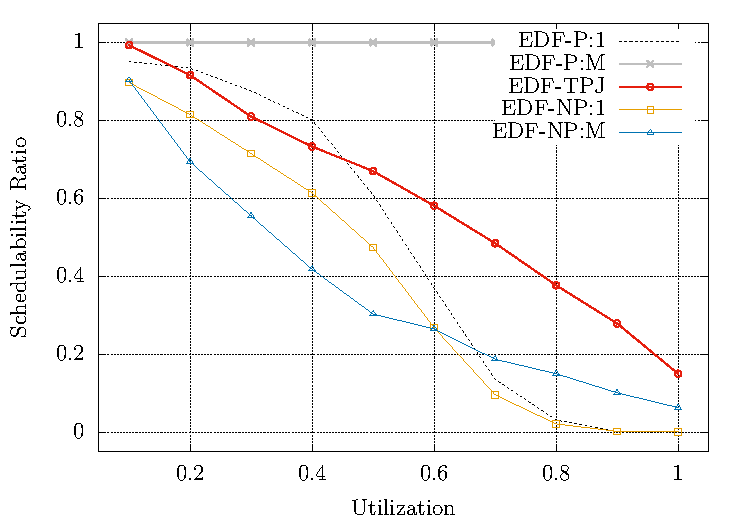
\includegraphics[width=\linewidth]{plot/cs-ratio/cs-ratio}
  \caption{\texttt{BUNDLEP} Case Study}
  \label{fig:cs-ratio}
\end{wrapfigure}

Figure~\ref{fig:cs-ratio} presents the results of the \bundlep{} case
study as a schedulability ratio for each of the schedulability test
combinations. For the target architecture and the specific benchmarks,
EDF-TPJ outperforms the other non-preemptive algorithms. EDF-TPJ
always outperforms EDF-NP:1 and performs better than or equal to
EDF-NP:M. Compared to the preemptive alternative EDF-P:1, EDF-TPJ
has consistently higher schedulability. 

%% \begin{wrapfigure}{l}{0.5\linewidth}
%%   \begin{subfigure}[t]{\linewidth}
%%     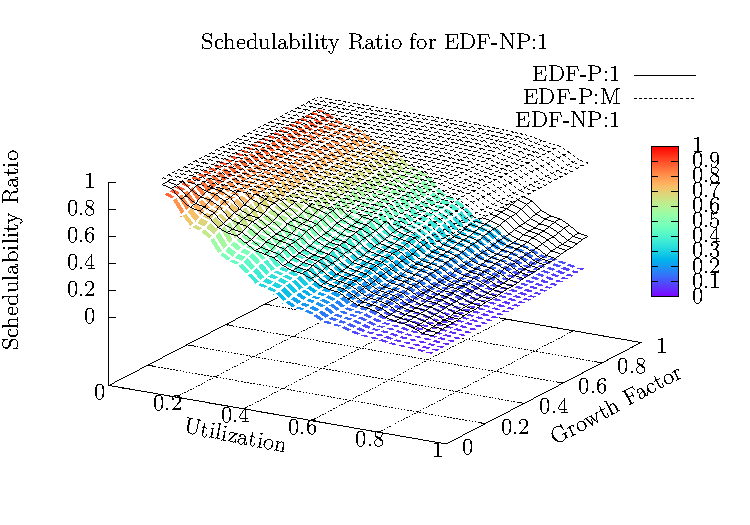
\includegraphics[width=\linewidth]{plot/avg-alg-sched/avg-ratio-NP-1}
%%   \end{subfigure}\\
%%   \begin{subfigure}[t]{\linewidth}
%%     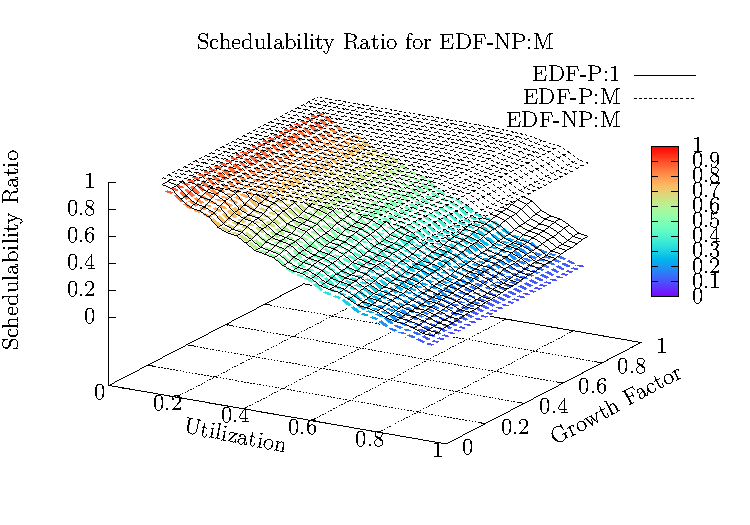
\includegraphics[width=\linewidth]{plot/avg-alg-sched/avg-ratio-NP-m}
%%   \end{subfigure}\\
%%   \begin{subfigure}[t]{\linewidth}
%%     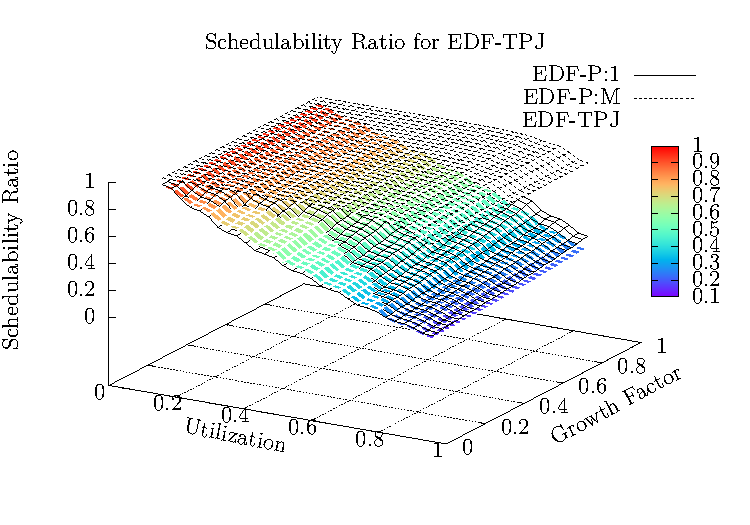
\includegraphics[width=\linewidth]{plot/avg-alg-sched/avg-ratio-TPJ-i}
%%   \end{subfigure}
%%   \caption{Schedulability Ratios}
%%   \label{fig:eval-summary}
%% \end{wrapfigure}

Figure~\ref{fig:eval-summary} summarizes the schedulability ratio
for the synthetic task set specifications, varying both
utilization and growth factor values. From top to bottom, the ratios
are presented for EDF-NP:1, EDF-NP:M, and EDF-TPJ. Within each graph, the
schedulability ratios provided by EDF-P:1 and EDF-P:M serve as
references. The difference between EDF-P:1 and the subject of the
graph illustrate the benefit of preemptive scheduling compared to the
non-preemptive scheduler. The difference between EDF-P:M and the
subject of the graph highlights the theoretical limit of concave
growth to schedulability. 

\begin{figure}[hb]
  \center
  \begin{subfigure}[t]{.32\linewidth}
    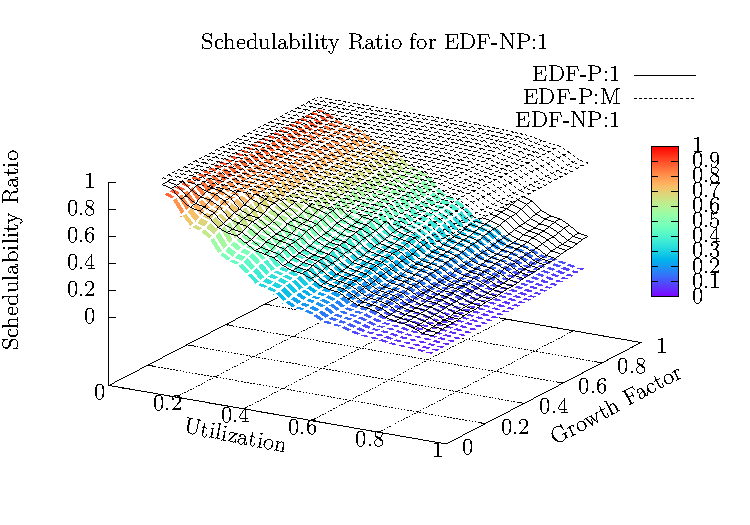
\includegraphics[width=\linewidth]{plot/avg-alg-sched/avg-ratio-NP-1}
  \end{subfigure}~
  \begin{subfigure}[t]{.32\linewidth}
    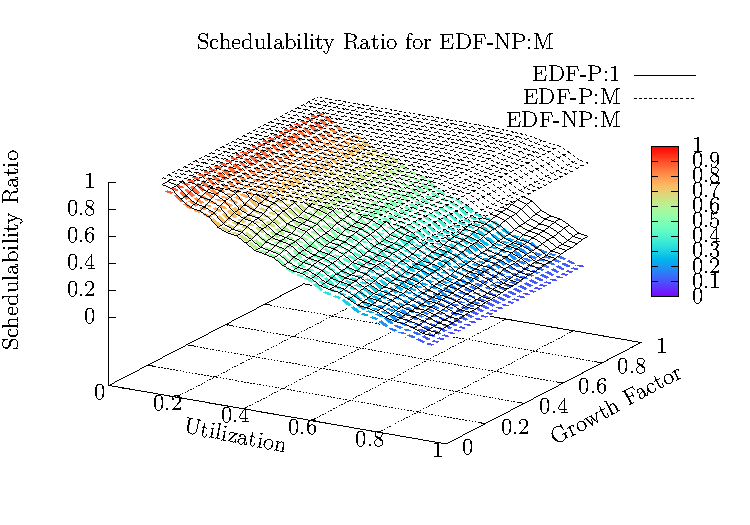
\includegraphics[width=\linewidth]{plot/avg-alg-sched/avg-ratio-NP-m}
  \end{subfigure}~
  \begin{subfigure}[t]{.32\linewidth}
    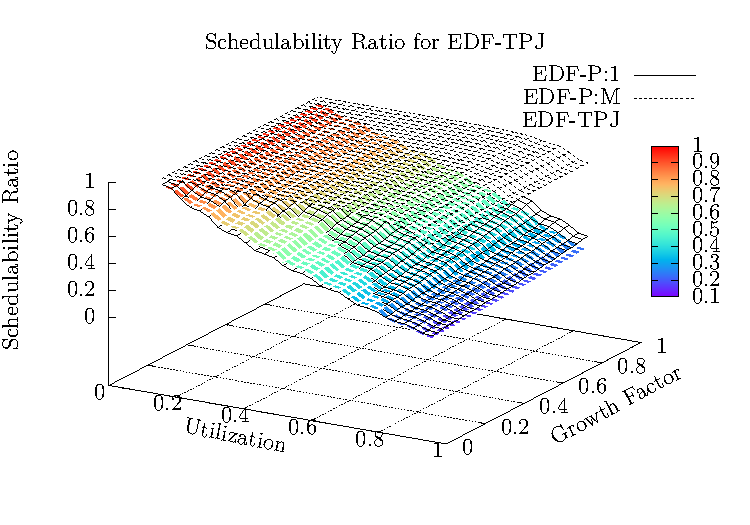
\includegraphics[width=\linewidth]{plot/avg-alg-sched/avg-ratio-TPJ-i}
  \end{subfigure}
  \caption{Schedulability Ratios}
  \label{fig:eval-summary}
\end{figure}

Including the surfaces of EDF-P:1 and EDF-P:M in all graphs of
Figure~\ref{fig:eval-summary} eases the comparison of scheduling
algorithms and schedulability tests. Comparing EDF-NP:1 
to EDF-NP:M, the benefits of the model and scheduling mechanism are
clear. EDF-NP:M has a consistently higher schedulability ratio for all
utilization and growth factor values. Outperforming
EDF-NP:M, EDF-TPJ has the highest schedulability ratios
over all utilization and growth factors due to the ability to
transform task sets. Additionally, EDF-TPJ is able to schedule task
sets deemed infeasible for EDF-P:1.

Table~\ref{table:by-m} summarizes the infeasible utilization
findings. For moderate and larger values of ${M \ge 25}$, the number
of infeasible by utilization task sets dominate the
specifications. For 25, 50, and 100 total threads, the infeasible by
utilization comprise 44, 59, and 74 percent of the task sets
respectively, with EDF-TPJ finding 25, 34, and 45 percent
feasible. This illustrates the large potential of the proposed model,
in conjunction with concave growth WCET functions of
thread-level schedulers (e.g. \bundle{} and \bundlep{}).

\begin{wraptable}{r}{.4\linewidth}
  \centering
  \input{../plot/over-one/by-m.tex}
\end{wraptable}

There are two noteworthy trends within the schedulability results.
The simpler of the two is the relationship between utilization and
schedulability ratio for a fixed growth
factor. Figure~\ref{fig:M10F.5} illustrates the trend common among 10
or fewer total threads. Unsurprisingly, the trend for preemptive and
non-preemptive schedulability tests when utilization increases is for the
schedulability ratio to decrease. However, EDF-TPJ always outperforms
the other non-preemptive tests. 

The second trend is slightly more complex. Figure~\ref{fig:M10U.5} was
selected as the smallest ${M}$ and ${U}$ values with distinct plots
for each schedulability test in the graph. The growth factor and the
schedulability ratio are correlated. As the growth factor increases,
so too does the schedulability ratio of all tests. This is due to
the utilization being held constant. When the growth factor is small,
the WCET of the first thread of each task is larger. Larger WCET values
are harder to schedule non-preemptively. Again, EDF-TPJ outperforms
all other non-preemptive tests across all configurations.

\begin{figure}[ht]
  \begin{subfigure}{.5\linewidth}
    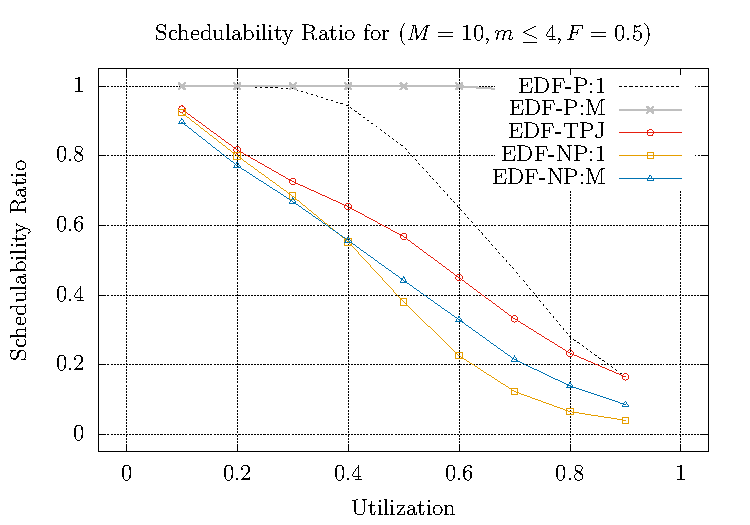
\includegraphics[width=\linewidth]{plot/2D-UFS/2D-M010m04F0_5xS}
    \caption{${(M,m,U,\GFactor{}) = (10,4,*,0.5)}$}
    \label{fig:M10F.5}
  \end{subfigure}%
  \begin{subfigure}{.5\linewidth}
    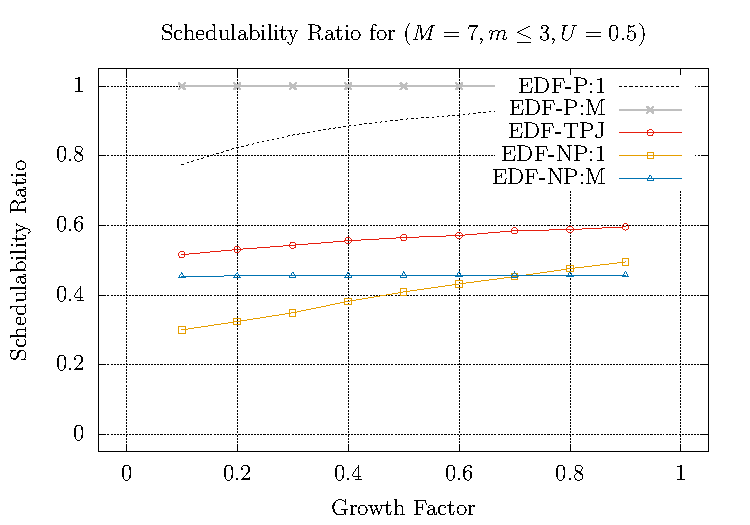
\includegraphics[width=\linewidth]{plot/2D-UFS/2D-M007m03U0_5xS.pdf}
    \caption{${(M,m,U,\GFactor{}) = (7,3,0.5,*)}$}
    \label{fig:M10U.5}
  \end{subfigure}
  \caption{${M \le 10}$ Performance}
\end{figure}

\begin{figure}[h]
  \begin{subfigure}[t]{.5\linewidth}
    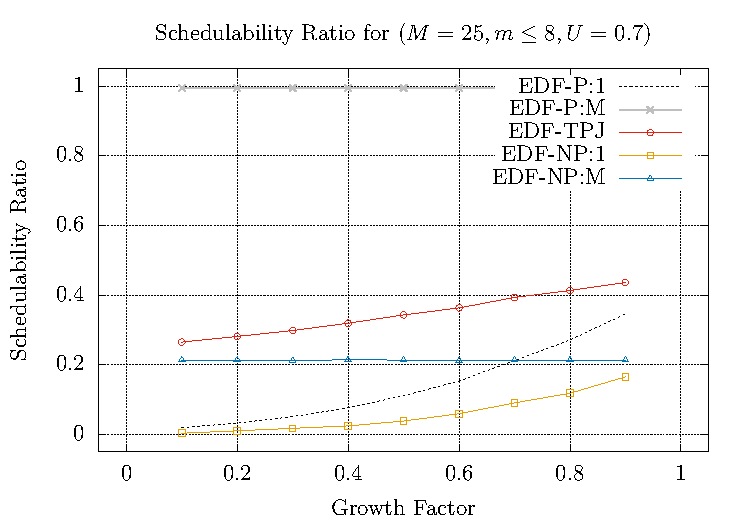
\includegraphics[width=\linewidth]{plot/2D-UFS/2D-M025m08U0_7xS}%
  \end{subfigure}%
  \begin{subfigure}[t]{.5\linewidth}
    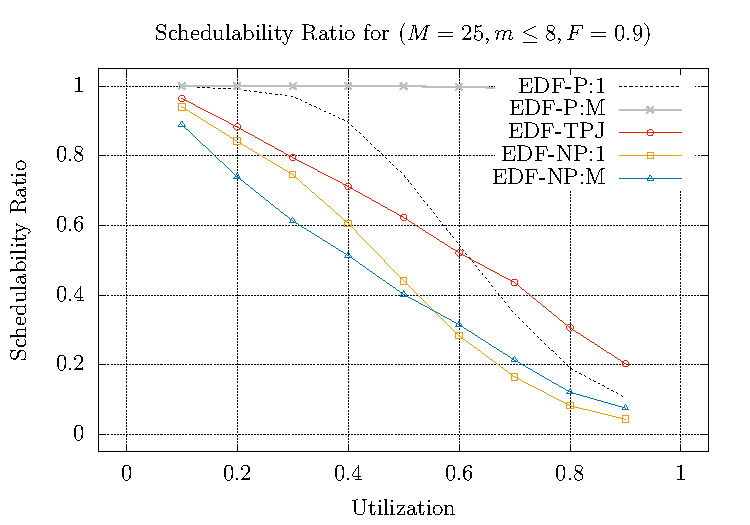
\includegraphics[width=\linewidth]{plot/2D-UFS/2D-M025m08F0_9xS}%
  \end{subfigure}%
  \caption{${M = 25}$ EDF-TPJ Performance Above EDF-P:1}
  \label{fig:m25-tpj}
\end{figure}

As ${M}$ increases beyond 10 total threads, the number of infeasible
by utilization task sets ${s}$ grows. This contributes to the
schedulability ratio of EDF-TPJ consistently surpassing EDF-P:1 for
minimum utilization and growth factor values. For ${M = 25}$, the
threshold of utilization is between ${[0.6,0.7]}$ shown in
Figure~\ref{fig:m25-tpj}.

For ${M = 100}$ when ${\GFactor \le 0.4}$ EDF-TPJ always outperforms
EDF-P:1. Figure~\ref{fig:m100-tpj} highlights the great advantage
EDF-TPJ has over EDF-P:1 by virtue of concave growth WCET
functions. It also highlights the advantage of dividing tasks, as the
performance of EDF-NP:M is always below EDF-TPJ.

\begin{figure}[ht]
  \begin{subfigure}[t]{.5\linewidth}
    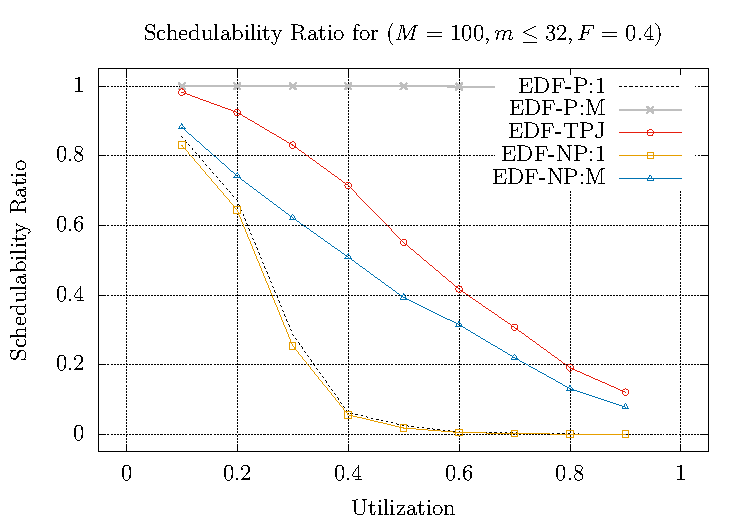
\includegraphics[width=\linewidth]{plot/2D-UFS/2D-M100m32F0_4xS}
%    \caption{${(M,m,U,\GFactor{}) = (100,32,*,0.4)}$}
  \end{subfigure}%
  \begin{subfigure}[t]{.5\linewidth}
    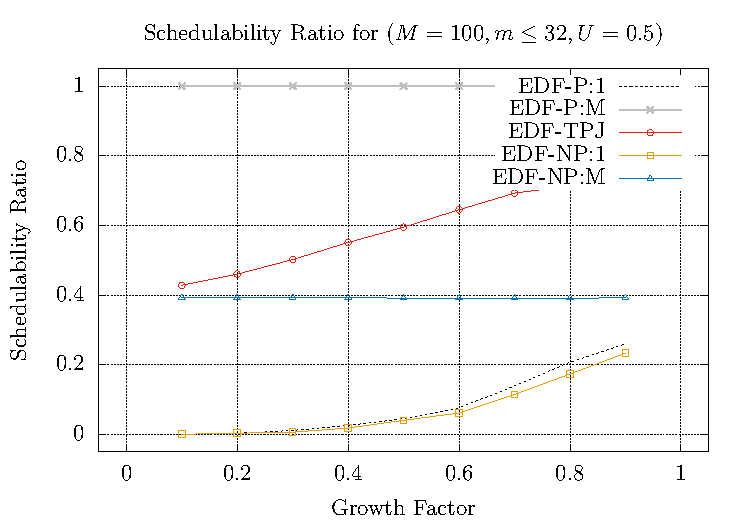
\includegraphics[width=\linewidth]{plot/2D-UFS/2D-M100m32U0_5xS}
%    \caption{${(M,m,U,\GFactor{}) = (100,32,0.5,*)}$}
  \end{subfigure}%
  \caption{${M = 100}$ EDF-TPJ Performance}
  \label{fig:m100-tpj}
\end{figure}

\begin{wrapfigure}{l}{.5\linewidth}
  \includegraphics[width=\linewidth]{plot/2D-UFS/2D-M003m02U0_7xS}
  \caption{${(M,m,U,\GFactor{}) = (3,2,0.7,*)}$}
  \label{fig:M3U.7}
\end{wrapfigure}

While EDF-TPJ always outperforms the other non-preemptive
schedulability tests, its distance from the non-preemptive tests is
least, and distance to EDF-P:1 the greatest for smaller values of
${M}$ and utilization above 0.4. Figure~\ref{fig:M3U.7}
illustrates the difference, where EDF-P:1 barely falls below 0.80, and
EDF-TPJ never rises to 0.40 for varying growth factors. EDF-TPJ
always outperforms EDF-NP:1 and EDF-NP:M, by a very small
amount. Suggesting the decrease in performance is more likely due to
the non-preemptive setting of EDF-TPJ, EDF-NP:1, and EDF-NP:M combined
with the larger WCET values for single threads.
